\problemname{Tågväxling}

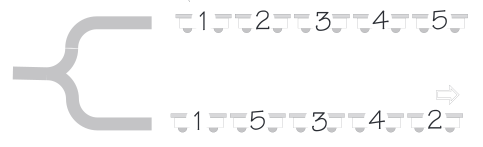
\includegraphics{tag.png}

På översta spåret (kallat inspåret) står ett tåg med $n \le 100$ vagnar, numrerade från 1 till $n$ med början från den främsta vagnen. På det undre spåret (kallat utspåret) ser du samma vagnar  önskad ordning då tåget lämnar växlingsområdet.

Ordningen mellan vagnarna kan förändras genom att köra upp dem på stickspåret (som är tillräckligt långt för att rymma alla vagnarna på en gång). Endast två förflyttningar är tillåtan.

\begin{itemize}
\item Första vagnen på inspåret till sista på stickspåret
\item Sista vagnen på stickspåret till sista på utspret
\end{itemize}
Skriv ett program som tar emot önskad ordning på utspåret och som avgör om denna ordning är möjlig att erhålla. Ordningen på de $n$ vagnarna på inspåret är alltid i stigande nummerordning från första till sista vagnen.

\section*{Indata}
Den första raden i indatan består av talet $n$.

Nästa rad består av $n$ heltal - den önskade ordningen på vagnarna.

\section*{Utdata}
Om det går att nå den önskade ställningen, skriv ut \texttt{JA}. Annars, skriv ut \texttt{NEJ}.
